\singlespacing

\mychapter{mygreen}{Méthodes}
	\sectiongreen*{Résumé}
		\begin{center}
			\begin{tabular}{c}
				\fcolorbox{mydarkgreen}{mylightgreen}{
				\begin{minipage}[][4cm][c]{0.8\linewidth}
					\sffamily
					Nous détaillerons ici notre méthode d'Intégration Transcriptome Interactome. J'ai choisi d'inclure dans cette section nos chapitres \citep{Garcia2011,Garcia2013}. Ces chapitres étant trop long, ils se trouvent dans les Annexes. Les données utilisées, ainsi que l'algorithme ITI\index{ITI} seront décrit en détail, et les outils utilisés seront décrits briévement.
				\end{minipage}}\\
				\\[2ex]
				\begin{minipage}[][4cm][c]{0.9\linewidth}
					\mtcsetdepth{minitoc}{1}
					\minitoc
				\end{minipage}
			\end{tabular}
		\end{center}
		\newpage

\doublespacing

	\section{\textcolor{mygreen}{Les avantages de l'intégration de données}}

		\subsection{\textcolor{mygreen}{Les avantages de l'intégration de données d'expression des gènes et d'interactions protéine-protéine}}
			\mylettrine{N}{ous} avons introduit dans le chapitre précédent les signatures prédictives dans le cancer du sein, ainsi que les limitations des technologies utilisées.
			Nous allons maintenant voir quels sont les avantages de l'intégration de données sur les performances de ces signatures.
			Reprenant les travaux de \citeauthor{vandevijver2002} et \citeauthor{Wang2005} sur l'analyse des jeux de données ayant permis l'établissement de signatures, \citeauthor{Chuang2007} rappellent les problèmes soulevés par ces prédentes études.

			Les ensembles de gènes permettant de prédire la rechute métastatique dans une étude sont moins efficaces quand il s'agit de prédire la rechute métastique sur le jeu de données de l'autre étude \citep{EinDor2006}.
			De plus, seulement trois gènes sont communs entre ces deux signatures à 70 et 76 gènes.
			L'hypothèse des gènes directeurs, à l'origine du cancer, pertubant les gènes en aval est reprise ici pour expliquer ces différences entre ces deux ensembles de gènes.
			Pour circonvenir à ces inconvénients, l'utilisation de données d'interaction protéine-protéine permet de combiner les mesures d'expression des gènes issus de réseaux communs.
			Les biomarqueurs permettant d'établir une signature ne sont dans ce cas là plus les gènes ou les protéines, mais des sous-réseaux de protéines interagissant ensemble au sein du réseau des interactions proteines-protéines humain.

			Cette méthode a des avantages par rapport aux analyses classiques :
			\begin{itemize}
				\item Les sous-réseaux résultants procurent des modèles des méchanismes moléculaires sous-jascents de la métastase.
				\item Les \emph{hubs} tels que \acs{TP53}, \acs{KRAS}, \acs{HRAS}, \acs{ERBB2}, non détectés par les analyses classiques, jouent un rôle central dans les réseaux en interconnectant un grand nombre de gènes.
				\item Les sous-réseaux identifiés sont signifiquativement plus reproductibles entre différentes études que des biomarqueurs individuels sélectionnés sans information sur les interactions protéine-protéine.
				\item Une classification basée sur des réseaux permet d'obtenir une prédiction plus précise en sélectionnant les marqueurs sur un premier jeu de données d'entraînement et en les appliquant à un deuxième jeu de données de validation indépendant (cf figure~\ref{fig:Chuang2007figS1}).
			\end{itemize}

			\begin{figure}
				\centering
				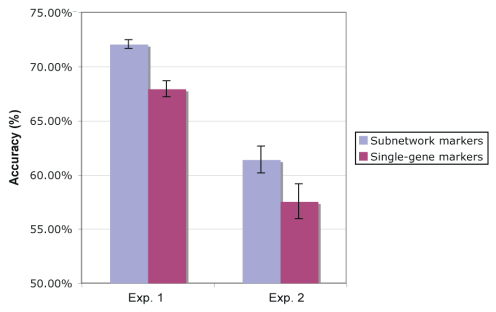
\includegraphics[width=\columnwidth]{figures/Chuang2007figS1.png}
				\caption{Avantages de l'intégration de données d'expression des gènes et d'interactions protéine-protéine sur la précision de la classification de la rechute métastatique par rapport à une analyse classique sur des données d'expression des gènes\citep{Chuang2007}.}
				\label{fig:Chuang2007figS1}
			\end{figure}

		\subsection{\textcolor{mygreen}{L'intégration de données d'expression des gènes et d'interactions protéine-protéine}}
			\mylettrine{C}{omme} nous venons de le détailler, cette méthode présente des avantages comparé aux méthodes classiques d'analyse de données d'expression des gènes.
			Nous allons détailler rapidement ici la méthode de \citeauthor{Chuang2007}.
			Plusieurs types de données sont nécessaires pour réaliser cette intégration.
			Il faut tout d'abord des données d'expression des gènes, ainsi que les données cliniques correspondantes, que nous détaillerons dans la partie ~\ref{sec:GEP}.
			Des données d'interactions protéine-protéine, que nous nous détaillerons dans la partie ~\ref{sec:IPP}, sont également indispensables.
			Elles sont utilisés pour assigner des ensembles de gènes sur des sous-réseaux.
			Les conditions cliniques des patients (\emph{ie} métastatique ou non-métastatique) permettent de différencier l'expression des gènes constituant les sous-réseaux pour constituer une matrice d'activité.
			Cette matrice d'activité sert à attribuer un score global à chaque sous-réseau, dérivé de l'expression de chacun des gènes le constituant.
			Des sous-réseaux générés par permutation permettent alors de sélectionner les sous-réseaux discrimants.
			Les sous-réseaux ainsi sélectionnés sont utilisés pour identifier les gènes causant la maladie, et la matrice d'activité du sous-réseau est utilisé pour entrainer un classifieur.

			\begin{figure}
				\centering
				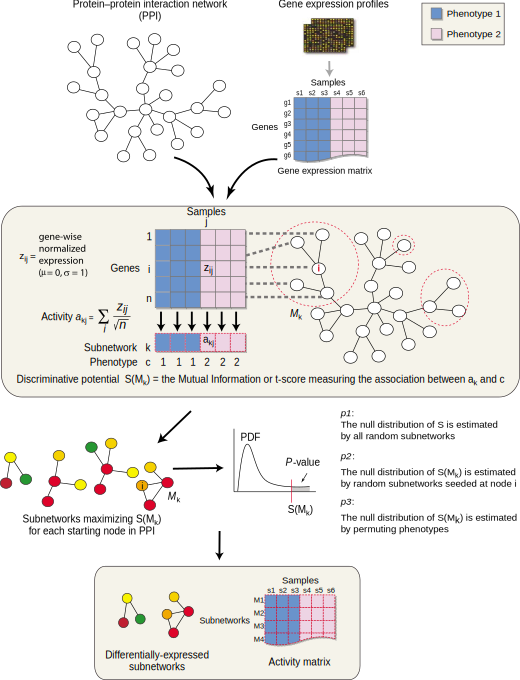
\includegraphics[width=\columnwidth]{figures/Chuang2007IntegrationAlgorithm.png}
				\caption{Algorithme détaillant l'intégration de données d'expression des gènes et d'interactions protéine-protéine\citep{Chuang2007}.}
				\label{fig:Chuang2007IntegrationAlgorithm}
			\end{figure}
		
	\section{\textcolor{mygreen}{L'\acl{ITIfr}}}

		\subsection{\textcolor{mygreen}{L'intégration massive de données d'expression des gènes et de données d'interactions protéine-protéine}}

			\mylettrine{L'}{intégration} massive de données d'expression des gènes et de données d'interactions protéine-protéine est la solution que nous avons dévelloppé pour circonvenir aux inconvénients des approches classiques des méthodes de prédiction de la rechute métastatique dans le cancer du sein.

			Nous avons vu précedemment que les approches classiques manquaient de reproductibilité, dépendaient grandement des jeux d'apprentissage et étaient moins performantes utilisées sur un jeu de données indépendant.

			Notre approche est une réimplémentation totale de l'algorithme développé par \citeauthor{Chuang2007}, avec la capacité supplémentaire de pouvoir prendre en compte plusieurs jeux de données d'expression des gènes.

			Nous allons d'abord détailler les données que nous avons utilisés tout au long de ces travaux.
			Et ensuite nous détaillerons l'algorithme.

	\section{\textcolor{mygreen}{Données d'expression des gènes}}\label{sec:GEP}

		\subsection{\textcolor{mygreen}{Constitution d'un compendium de données d'expression des gènes dans le cancer du sein}}
			\mylettrine{N}{ous avons} exploré les sites de dépôts de données publiques, ainsi que la littérature, et avons sélectionné les jeux de données dont les conditions cliniques étaient disponibles.
			\begin{table}
				\begin{center}
					\caption{Liste des jeux de données inclus dans notre compendium de données d'expression dans le cancer du sein.}
					\begin{tabular}{llccc}
						\toprule
						\multirow{3}{3cm}{\emph{Jeu de données}} & \multirow{3}{2cm}{\emph{Plateforme}} & \multirow{3}{2cm}{\centering\emph{Nombre d'échantillons}} & \multirow{3}{2cm}{\centering\emph{Présence de données cliniques}} \\
										&									&		&		\\
										&									&		&		\\
						\midrule
						Anders			& U95v2								& 78	& Non	\\
						Bild			& U95v2								& 158	& Non	\\
						Campone			& UMGC-IRCNA 9k A					& 150	& Non	\\
						Chang			& cDNA array						& 50	& Non	\\
						Chang-Kyu		& Merck GEL Breast Tumor Profiles	& 311	& Non	\\
						Chanrion		& MLRG Human 21K V12.0				& 155	& Non	\\
						Desmedt			& U133A								& 198	& Oui	\\
						Ivshina			& U133 Plus 2.0						& 289	& Oui	\\
						Jezequel		& UMGC-IRCNA 9k A					& 252	& Non	\\
						Kreike			& NKI-AVL 18K cDNA					& 59	& Oui	\\
						Loi				& U133A + U133B						& 327	& Oui	\\
										& U133 Plus 2.0						& 87	& Oui	\\
						Miller			& U133A + U133B						& 251	& Oui	\\
						Parker			& Agilent-011521 1A G4110A			& 2		& Oui	\\
										& Agilent-012097 1A G4110B			& 27	& Oui	\\
										& Agilent 1A Oligo UNC Custom		& 196	& Oui	\\
						Pawitan			& U133A + U133B						& 159	& Oui	\\
						Perou			& SCV								& 84	& Non	\\
						Sabatier		& U133 Plus 2.0						& 129	& Oui	\\
						Schmidt			& U133A								& 200	& Oui	\\
						S{\o}rlie		&									& 85	& Non	\\
						Sotiriou		& U133A								& 189	& Oui	\\
						van de Vijver	& Agilent whole human genome		& 295	& Oui	\\
						van't Veer		& Agilent whole human genome		& 117	& Oui	\\
						Wang			& U133A								& 286	& Oui	\\
						Wong			& U133A								& 6		& Non	\\
						Yu				& U133A								& 341	& Non	\\
						Zhang			& U133A								& 136	& Oui	\\
						Zhou			& U133Av2							& 54	& Oui	\\
						\midrule
						Total			& 7 différentes						& 2572	&		\\
						\bottomrule
					\end{tabular}
					\label{tab:MetDatasets}
					\vspace{5ex}
					\caption*{Tous les jeux de données présentés ici ont été considérés, cependant nous avons gardé seulement les jeux de données accompagnés de données cliniques. Les jeux de données rejetés pourraient cependant être inclus si les données cliniques étaient accessibles.}
				\end{center}
			\end{table}

			Nous avons téléchargé sur Gene Expression Omnibus, ou sur le site dédié de l'auteur l'ensemble des jeux de données. Si cela était possible nous avons téléchargé les données brutes, et avons réalisé une normalisation gcrma (package affy du package bioconductor) via R.

			Nous avons utilisé ces jeux de données d'expression dans le cancer du sein pour deux analyses.
			Pour la première analyse, non supervisée, nous avons uniquement utilisé comme données cliniques l'événement DMFS.
			Voici les jeux de données que nous avons finalement utilisés pour notre première analyse (\emph{cf} ~\ref{chap:results1}).

			\begin{table}
				\begin{center}
					\caption{Liste des jeux de données inclus pour notre analyse non supervisée \citep{Garcia2011} (\emph{cf} ~\ref{chap:results1}).}
					\begin{tabular}{lccc}
						\toprule
						\multirow{2}{3cm}{\emph{Jeu de données}}	& \multirow{2}{3cm}{\centering\emph{Nombre d'échantillons}}	& \multirow{2}{3cm}{\centering\emph{Nombre de status \acs{DMFS} positif}} & \multirow{2}{3cm}{\centering\emph{Nombre de status \acs{DMFS} négatif}} \\
									&									&		&		\\
						\midrule
						Desmedt						& 198	& 62	&	136		\\
						\citep{Desmedt2008}			&		&		&			\\
						Ivshina						& 249	& 89	&	160		\\
						\citep{Ivshina2006}			&		&		&			\\
						Loi							& 117	& 26	&	91		\\
						\citep{Loi2008}				&		&		&			\\
						Parker						& 199	& 45	&	154		\\
						\citep{Parker2009}			&		&		&			\\
						Pawitan						& 159	& 40	&	119		\\
						\citep{Pawitan2005}			&		&		&			\\
						Schmidt						& 200	& 46	&	154		\\
						\citep{Schmidt2008}			&		&		&			\\
						Sabatier					& 31	& 9		&	22		\\
						\citep{Sabatier2011}		&		&		&			\\
						Sotiriou					& 179	& 40	&	139		\\
						\citep{Sotiriou2009}		&		&		&			\\
						van de Vijver				& 295	& 88	&	207		\\
						\citep{vandevijver2002}		&		&		&			\\
						Wang						& 286	& 107	&	179		\\
						\citep{Wang2005}			&		&		&			\\
						Zhang						& 136	& 20	&	116		\\
						\citep{Zhang2009a}			&		&		&			\\
						Zhou						& 54	& 9		&	45		\\
						\citep{Zhou2007}			&		&		&			\\
						\midrule
						Total						& 2103	& 581	&	1522	\\
						\bottomrule
					\end{tabular}
					\label{tab:Met:DSNS}
					\vspace{5ex}
					\caption*{L'utilisation de 12 jeux données nous donne l'accès à plus de 2000 tumeurs pour notre analyse non supervisée.}
				\end{center}
			\end{table}

			Pour notre seconde analyse, supervisée, nous avons choisi par soucis d'homogénéisation de ne sélectionner que les patientes sans traitements supplémentaires, et ainsi éviter de séparer les patientes en fonction de la réponse au traitement.
			Dans les données cliniques nous récupérions également les expressions des \aclp{ER}.
			Dans le but d'avoir un ensemble d'échantillons le plus homogène possible, nous les avons soigneusement choisi en nous basant sur les données cliniques accessibles.
			Toutes les informations cliniques ont été téléchargés sur \acs{GEO} le site de dépôt de bases de données publiques du \acs{NCBI}, pour les jeux de données préalablement récupérés sur ce même site \citep{Desmedt2008, Loi2008, Sabatier2011, Schmidt2008, Wang2005}, ou sur le site internet de l'auteur\footnote{\url{bioinformatics.nki.nl/data.php}} pour le jeu de données de van de Vijver \citep{vandevijver2002}.
			Les données cliniques qui nous intéressaient, étaient :
			\begin{itemize}
				\item Le status \acs{DMFS}
				\item Le temps de mesure de ce status \acs{DMFS}
				\item Le status \acs{ER}
				\item La présence ou non de traitement, et sa nature éventuelle
				\item La présence ou non de ganglions, et leur nombre éventuel
			\end{itemize}

			\begin{table}
				\begin{center}
					\caption{Liste des jeux de données inclus pour notre analyse supervisée \citep{Garcia2012} (\emph{cf} ~\ref{chap:results2}).}
					\begin{tabular}{llr@{/}lr@{/}lr@{/}l}
						\toprule
						\emph{Jeu de données} & \emph{Plateforme}	& \multicolumn{2}{c}{\emph{Nombre d'échantillons}}	& \multicolumn{2}{c}{\emph{Statuts DMFS}} & \multicolumn{2}{c}{\emph{Statuts ER}} \\
						\cmidrule(r){3-8}
						&  & \emph{(Sélectionnés} & \emph{Total)}	& \emph{(meta} & \emph{non meta)} & \emph{(ER-}	& \emph{ER+)} \\
						\midrule
						Desmedt						& U133A												& 190	&198	& 62	& 128	& 61	& 129	\\
						Loi							& U133A + U133B										& 101	&327	& 27	& 74	& 29	& 72	\\
						Sabatier					& U133 Plus 2.0										& 31	&255	& 9		& 22	& 11	& 20	\\
						Schmidt						& U133A												& 182	&200	& 46	& 136	& 37	& 145	\\
						van de Vijver				& \multirow{2}{2.49cm}{Agilent whole human genome}	& 150	&295	& 56	& 94	& 36	& 114	\\
						& \\
						Wang						& U133A												& 276	&286	& 107	& 169	& 72	& 204	\\
						\midrule
						Total						& 7 différentes										& 930	&1561	& 307	& 623	& 246	& 684	\\
						\bottomrule
					\end{tabular}
					\label{tab:Met:DSS}
					\vspace{5ex}
					\caption*{L'utilisation de 6 jeux données nous donne l'accès à plus de 1500 tumeurs pour notre analyse supervisée.}
				\end{center}
			\end{table}

			Après avoir détaillé les jeux de données, leur constitutions

	\section{\textcolor{mygreen}{Interactions protéine-protéine}}\label{sec:IPP}

		\subsection{\textcolor{mygreen}{Assemblage d'interactomes humains}}
			\mylettrine{L}{a} biologie moléculaire décrit les différents constituants de la cellule (protéines, \acs{ADN}, \acs{ARN} et autres molécules). Mais un organisme vivant est une entité complexe, et il est difficile de le comprendre totalement en analysant des parties spécifiques. C'est pour cela que l'on envisage l'organisme comme un système ou un réseau d'interactions.
			Les protéines interagissent les unes avec les autres dans une cellule, et ces interactions donnent lieu à des fonctions biologiques et un comportement dynamique du système cellulaire. Généralement ces interactions protéine-protéine sont temporelles, spatiales, ou dépendantes d'une condition spécifique.
			L'un des plus grands enjeux dans l'ère post-génomique de la biologie est de récolter des informations d'interactions entre protéines, \acsp{ADN} et autres petites molécules, et de comprendre comment ces interactions sont organisées.
			Les techniques à haut débit ont permis la génération d'un grand nombre de données d'interactions protéine-protéine.
			Pour \acs{ITIfr} nous avons récupéré différentes bases de données d'interactions protéine-protéine.

		\subsection{\textcolor{mygreen}{Nature des interactions et bases de données d'interactions utilisées}}
			\mylettrine{L}{es} interactions contenues dans les bases de données d'interactions protéine-protéine sont récoltés par différentes techniques, et sont également de différente nature.
			Nous considérons commes sûres les interactions décrites dans la littérature et celle vérifiées par une technique de double hybride dans la levure.
			Les interactions de complexes par Co-immuno-précipitation ne sont pas directes, mais concernent des protéines qui font parties d'un même complexe.
			Enfin, les interactions sont des prédictions obtenues par divers algorithmes, et ne sont pas vérifiés.
			Elles sont donc moins sûres que les autres interactions. 

			HPRD \citep{Prasad2009}, INTAct \citep{Aranda2010}, DIP \citep{Xenarios2000} et MINT \citep{Zanzoni2002} contiennent des interactions décrites dans la littérature et vérifiées par double hybride.
			CORUM \citep{Ruepp2008} contient des interactions de complexes.
			Cocite \citep{Ramani2005} contient des interactions prédites in silico.


	\section{\textcolor{mygreen}{Données et outils supplémentaires}}
		\mylettrine{N}{ous} utilisons également des données supplémentaires pour les besoins de notre algorithme.
			Pour l'annotation des différentes plateformes de puces à \acs{ADN}, nous utilisons les fichiers fournis par Resourcerer \citep{Tsai2001}.
			Pour l'annotation des gènes, nous utilisons le fichier Homo\_sapiens.gene\_info.gz fourni par le \acs{NCBI}\footnote{\url{ftp://ftp.ncbi.nlm.nih.gov/gene/DATA/GENE_INFO/Mammalia/}}.

			Nous avons également utilisés des outils supplémentaires pour la vizualisation et les analyses de nos résultats.
			Pour visualiser nos sous-réseaux, nous avons utilisé le logiciel libre Graphviz\footnote{\url{http://graphviz.org/}} développé par AT\&T Research et le modèle de rendu neato.
			Pour analyser l'enrichissement en terme GO, nous avons utilisé le programme ErmineJ \citep{Gillis2010}.
			Pour notre analyse supervisée ~\ref{chap:results2} nous utilisons la librarie libSVM \citep{Chang2007} pour classifier nos échantillons.

	\pagebreak

	\section{\textcolor{mygreen}{Algorithme}}

		\subsection{\textcolor{mygreen}{Détection des sous-réseaux}}
			\mylettrine{L}{a première} étape de notre algorithme est la détection de sous-réseaux.
			Les données utilisées par \acs{ITIfr} en entrée sont d'une part des données d'expressions des gènes, ainsi que les conditions cliniques correspondantes aux patients, et des données d'interactions protéine-protéine que nous avons détaillés précédemment (données d'expressions des gènes \ref{sec:GEP}, données d'interactions protéine-protéine \ref{sec:IPP}).
			Les données d'interactions protéine-protéine sont rassemblées pour ne former qu'un seul interactome.
			Les interactions d'une protéine vers elle même n'ont pas été gardées.
			Nous avons gardés les interactions en nous basant sur l'unicité de l'identifiant gene ID fourni par les fichiers d'annotations du NCBI. 
			Les données d'expressions des gènes sont considérées séparément pour chacun des jeux de données utilisés.
			Chaque gène est utilisé successivement comme graine pour créer un sous-réseau.
			Ce processus est parallèlisé sur un cluster de calcul de type BEOWULF.
			Pour chacun des jeux de données d'expression des gènes, la corrélation des conditions cliniques avec les \acs{GEP} est calculé.
			Ainsi, si un gène n'a pas d'expression dans un jeu de données particulier, à cause des différences entre les plateformes, il peut quand même être pris en compte pour la constitution d'un sous-réseaux.
			Récursivement nous considérons le premier voisin du gène graine, et l'ajoutons à notre sous-réseau en construction, si l'ajout de ce gène améliore le score du sous-réseau, suivant l'équation \ref{eq:score} :
			\begin{equation}\label{eq:score}
				S_{s,d}=\frac{\sqrt{n_{d}}}{\sqrt{\max n_{d}(DS)}}\Bigg|corr\Bigg(\frac{1}{n}\sum_{g\in S}e(g,d),cc(d)\Bigg)\Bigg|
			\end{equation}
			Le score du sous-réseaux étant calculé en fonction de la corrélation entre les conditions cliniques et les \acs{GEP}.
			Au fur et à mesure de l'ajout de gènes au sous-réseau, l'apport d'un nouveau gène peut n'augmenter que de très peu le score du sous-réseau.
			C'est pourquoi nous avons ici mis une valeur de seuil pour l'amélioration des sous-réseaux.

			Un score global, non utilisé pour le calcul, mais pour simplifier l'affichage des résultats est calculé en faisant la moyenne des scores sur les différents jeux de donnés d'expression utilisés, suivant l'équation \ref{eq:global} :
			\begin{equation}\label{eq:global}
				S_{s}=\frac{1}{NS}\sum_{d\in DS}S(s,d)
			\end{equation}

			\begin{figure}
				\begin{center}
					\def\svgwidth{\columnwidth}\input{figures/Algorithme.pdf_tex}
					\caption{Principe de la sélection des sous-réseaux avec \acl{ITIfr}.}
					\label{fig:Algorithme}
				\end{center}
			\end{figure}
			
			Reprenant cette étape de détection des sous-réseaux, nous construisons, dans le but de valider statistiquement les sous-réseaux que nous venons de détecter, des sous-réseaux de manière aléatoires.
			Nous allons détailler cette étape dans la prochaine partie.

		\subsection{\textcolor{mygreen}{Validation statistique}}
			\mylettrine{N}{ous utilisons} trois méthodes pour générer des sous-réseaux aléatoires, se basant sur le principe de construction de sous-réseaux expliqué précédement.
			Premièrement, nous mélangeons les conditions cliniques, et essayons de détecter des sous-réseaux.
			Secondement, la décision d'ajout d'un gène à un sous-réseau ne dépend plus de la corrélation des conditions cliniques avec les \acs{GEP}, mais est aléatoire.
			Troisièment, nous mélangeons nos interactions protéines-protéines, et essayons de détecter des sous-réseaux.
			Ces trois méthodes différentes nous permettent de générer trois ensemble de sous-réseaux qui vont servir pour valider statistiquement les véritables sous-réseaux détectés précédemment.
			Pour garder les ensembles des sous-réseaux aléatoires comparables avec les sous-réseaux détectés, les distributions de leurs tailles sont forcés pour correspondre à celle des sous-réseaux détectés par modèle gaussien.
			Les distributions des scores des sous-réseaux aléatoires sont modelés par mixture de deux distributions gaussiennes.
			Ces distributions sont utiliser pour fixer des seuils sur les scores, indépendamment des jeux de donnés d'expression, et ainsi leurs attribuer des p-values.
			Le mélange des interactions protéine-protéines ne permet pas de génerer un nombre important de sous-réseaux, confirmant l'importance du lien entre les intéractions protéines-protéines et le niveau d'expression des gènes.
			La validation statistique est réalisée avec Matlab Statistical Toolbox R2010b.

		\subsection{\textcolor{mygreen}{Sélection de sous-réseaux}}
			\mylettrine{L}{es p-values} calculées lors de l'étape de validation statistique sont utilisées pour filtrer les sous-réseaux détectés statistiquement significatifs.
			Les distributions des trois ensembles de sous-réseaux aléatoires nous ont permis d'attribuer 3 p-values différentes pour chacun des sous-réseaux.
			Nous sélectionnons un seuil de p-value pour chacune des distributions aléatoires et l'utilisons pour filtrer les sous-réseaux détectés et générons trois ensembles de sous-réseaux stastitiquement significatifs suivant chacune des méthodes précédemment expliquées.
			Nous réalisons alors l'intersection de ces trois ensemble pour constituer un ensemble de sous-réseaux dont la significativité est validé par trois distributions aléatoires.
			Pour faciliter l'affichage et l'interprétation des résultats, nous combinons les trois différentes p-values avec la méthode de Fisher \citep{Fisher1925}.
			Cet ensemble final de sous-réseaux constitue une signature avec laquelle nous pourrons classifier des échantillons et ainsi comparer la performance des signatures trouvées avec notre méthode ITI et les autres méthodes existantes.
			Nous détaillerons ces résultats dans la partie ~\ref{chap:results2}.
			Nous allons maintenant détailler la réalisation d'une ressource bioinformatique contenant les différents sous-réseaux trouvés lors de nos analyses.

		\subsection{\textcolor{mygreen}{Création d'une ressource bioinformatique permettant l'analyse des sous-réseaux}}
			\mylettrine{P}{our permettre} le parcours des différents ensembles de sous-réseaux trouvés lors de nos analyses, nous avons créé une ressource bioinformatique permettant, l'affichage, l'interprétation et l'analyse des sous-réseaux.
			Cette ressource est accessible par internet, et constitue le site internet companion de nos publications \footnote{\url{http://iti.sourceforge.net/}}.
			Dans un soucis de reproductibilité de la recherche, le code source du projet \ac{ITIfr} est disponible sous licence CeCILL sur sourceforge \footnote{\url{http://sourceforge.net/projects/iti/}}.
			Chaque analyse est présentée.
			Pour chaque analyse nous avons accès aux sous sous-réseaux détectés statistiquement significatifs.
			Une page présente chacun des sous-réseaux.
			Nous avons utilisé le modèle de rendu neato du logiciel GraphViz pour permettre l'affichage des sous-réseaux.
			Une image en format png est générée par jeux de données d'expression pour chacun des sous-réseaux.
			Les scores et les p-values du sous-réseau en fonction du jeu de données d'expression permet de vérifier la significativité des sous-réseaux.
			Pour chacun des gènes du sous-réseau se trouve la valeur de la corrélation des conditions cliniques avec son expression pour chacun des jeux de données d'expression.
			Pour chacun des gènes, un lien vers la page du gène sur le site du NCBI est fournie, et permet d'utiliser les ressources du NCBI pour analyser plus en détail le gène.
			Pour permettre plus facilement la navigation d'un sous-réseau à un autre, pour chaque gène il existe une page listant les sous-réseaux dans lesquels il apparait.
			Enfin, pour chacun des sous-réseaux un enrichissement en terme GO est calculé, par jeux de données d'expression, se basant sur l'apport des gènes du sous-réseaux par rapport à l'ensemble des gènes présents sur la plateforme de puce à \acs{DNA} utilisée pour constituer le jeu de données.


	\section{\textcolor{mygreen}{Conclusion}}
		\mylettrine{A}{près} avoir détaillé notre méthode, nous allons maintenant présenter les résultats que nous avons obtenus. Tout d'abord, nous allons détailler nos résultats sur une analyse non-supervisée~\ref{chap:results1}, puis par la suite nous allons détailler nos résultats sur une analyse supervisée~\ref{chap:results2}.